%----------------------------------------------------------------------------------------
%	PACKAGES AND OTHER DOCUMENT CONFIGURATIONS
%----------------------------------------------------------------------------------------

\documentclass[11pt]{scrartcl} % Font size

\input{structure.tex} % Include the file specifying the document structure and custom commands
\usepackage{multirow}
\usepackage{array}
\usepackage{subcaption}
% Bar chart drawing library 
\usepackage{pgfplots} 
\usepackage{textcomp}
\usepackage{algorithm}
\usepackage{algpseudocode}

% Define a macro to create a table with fixed column widths
\newcolumntype{C}[1]{>{\centering\arraybackslash}p{#1}}

\usepackage{hyperref}
\hypersetup{
    colorlinks=true,
    linkcolor=blue,
    filecolor=magenta,      
    urlcolor=cyan,
}

\definecolor{codegreen}{rgb}{0,0.6,0}
\definecolor{codegray}{rgb}{0.5,0.5,0.5}
\definecolor{codepurple}{rgb}{0.58,0,0.82}
\definecolor{backcolour}{rgb}{0.95,0.95,0.92}
\definecolor{codeblue}{rgb}{0,0,0.8}

\lstdefinestyle{mystyle}{
    backgroundcolor=\color{backcolour},   
    commentstyle=\color{codegreen},
    keywordstyle=\color{codeblue},
    numberstyle=\tiny\color{codegray},
    stringstyle=\color{codepurple},
    basicstyle=\ttfamily\footnotesize,
    breakatwhitespace=false,         
    breaklines=true,                 
    captionpos=b,                    
    keepspaces=true,                 
    numbers=left,                    
    numbersep=5pt,                  
    showspaces=false,                
    showstringspaces=false,
    showtabs=false,                  
    tabsize=2
}

\lstset{style=mystyle}

\newcommand{\showpcaimage}[1]{
    \begin{figure}[H]
        \centering
        \begin{subfigure}[b]{0.45\textwidth}
            \includegraphics[width=\textwidth]{./assets/#1_1.jpg}
            \caption{Ποσοστό από Principal Components -- 1\%}
        \end{subfigure}
        \begin{subfigure}[b]{0.45\textwidth}
            \includegraphics[width=\textwidth]{./assets/#1_25.jpg}
            \caption{Ποσοστό από Principal Components -- 25\%}
        \end{subfigure}
        \begin{subfigure}[b]{0.45\textwidth}
            \includegraphics[width=\textwidth]{./assets/#1_75.jpg}
            \caption{Ποσοστό από Principal Components -- 75\%}
        \end{subfigure}
        \begin{subfigure}[b]{0.45\textwidth}
            \includegraphics[width=\textwidth]{./assets/#1_100.jpg}
            \caption{Ποσοστό από Principal Components -- 100\%}
        \end{subfigure}
        \caption{Ποσοστό από Principal Components που κρατήσαμε. Εικόνα \src{#1}}
    \end{figure}
}

%----------------------------------------------------------------------------------------
%	TITLE SECTION
%----------------------------------------------------------------------------------------

\title{	
	\normalfont\normalsize
	\textsc{Πανεπιστήμιο Πατρών, Τμήμα Μηχανικών ΗΥ και Πληροφορικής}\\ % Your university, school and/or department name(s)
	\vspace{25pt} % Whitespace
	\rule{\linewidth}{0.5pt}\\ % Thin top horizontal rule
	\vspace{20pt} % Whitespace
    {\LARGE Λογισμικό και Προγραμματισμός Συστημάτων Υψηλής Επίδοσης\\ Άσκηση 3 - CUDA \& OpenACC}\\ % The assignment title
	\vspace{12pt} % Whitespace
	\rule{\linewidth}{2pt}\\ % Thick bottom horizontal rule
	\vspace{12pt} % Whitespace
}


\author{Ευάγγελος Λάμπρου \\UP1066519 \and Ιωάννης Παναρίτης \\UP1072632} % Your name

\date{} % Today's date (\today) or a custom date

%----------------------------------------------------------------------------------------
%	DOCUMENT
%----------------------------------------------------------------------------------------

\bibliographystyle{abbrv}
\addto\captionsgreek{\renewcommand{\refname}{Αναφορές}}

\begin{document}

\maketitle 

\section{CUDA}

\subsection{Υλοποίηση}

Για την υλοποίηση αυτής της άσκησης έγινε παραλληλισμός των βημάτων του \src{Diffusion2D} με χρήση \src{CUDA} σε GPU.\\
Συγκεκριμένα, έχουμε τα εξής βήματα:

\begin{enumerate}
    \item Κατά την δημιουργία του αντικειμένου Diffusion2D, γίνεται allocate και μηδενισμός των πινάκων σε device memory.
    \item Αντιγραφή του πίνακα \src{rho} από host σε device
    \item Κάλεσμα της \src{PropagateDensity}. Εδώ επιλέγουμε τις διαστάσεις που θα έχουμε στην gpu και καλούμε το \src{diffusion\_kernel}.
    \item Κάθε thread της gpu εκτελείται παράλληλα. Ανάλογα με το id του, υπολογίζει τις καινούριες τιμές για το αντίστοιχο κελί του πίνακα \src{d\_rho}.
    \item Συγχρονισμός των threads του device.
    \item Αντιγραφή των δεδομένων στον host για αποθήκευση.
\end{enumerate}

Με τον perf profiler φαίνεται πως η πλειονότητα του χρόνου σπαταλάται στην συνάρτηση \src{Diffusion2D::PropagateDensity}.

\lstinputlisting[caption=Αποτελέσματα του perf report.]{assets/report_diffusion.txt}

\subsection{Μετρήσεις}

Οι παρακάτω μετρήσεις έγιναν σε σύστημα με επεξεργαστή \src{AMD Ryzen 7 2700 Eight-Core Processor @ 3.20 GHz} και κάρτα γραφικών \src{NVIDIA GeForce GTX 1660 6GB}.

% create a bar plot of the above time measurements using tikz. make it a centered figure with a caption.
\begin{figure}[H]
    \begin{center}
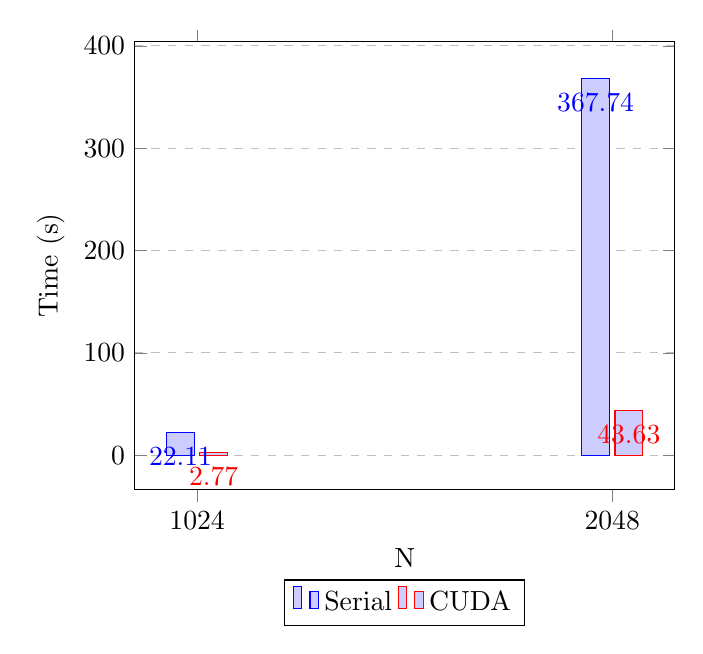
\begin{tikzpicture}
    \begin{axis}[
        xlabel={N},
        ylabel={Time (s)},
        xtick=data,
        xticklabels={1024, 2048},
        ybar,
        enlarge x limits=0.15,
        bar width=10pt,
        legend style={at={(0.5,-0.20)}, anchor=north, legend columns=-1},
        legend entries={Serial, CUDA},
        ymajorgrids=true,
        y grid style=dashed,
        nodes near coords,
        nodes near coords align={vertical},
        nodes near coords style={anchor=north},
        every node near coord/.append style={yshift=-2pt},
        every axis plot post/.append style={fill=blue!20},
        ]
        \addplot coordinates {(1024, 22.1073) (2048, 367.739)};
        \addplot coordinates {(1024, 2.76905) (2048, 43.6307)};
    \end{axis}
\end{tikzpicture}
    \end{center}
    \caption{Χρόνοι εκτέλεσης της υλοποίηση με και χωρίς CUDA.}
    \label{fig:cuda_times}
\end{figure}

\subsection{Έλεγχος Αποτελεσμάτων}

\begin{lstlisting}[language=Bash]
$ diff Density_cu_1024.dat Density_seq_1024.dat > diffs.dat
$ cat diffs.dat | head -n 8
20c20
< -1	-0.962854	9.70025e-09
---
> -1	-0.962854	9.70024e-09
50c50
< -1	-0.904203	4.39741e-08
---
> -1	-0.904203	4.3974e-08
\end{lstlisting}

Βλέπουμε τα αποτελέσματα είναι σωστά, αφού οι τελικές τιμές των κελιών είναι ίδιες με μεγάλη ακρίβεια 
μεταξύ των δύο υλοποιήσεων.
Η απόκλιση πιθανότατα οφείλεται στη διαφορετική σειρά εκτέλεσης των floating point operations.

\section{OpenACC}

\subsection{Υλοποίηση}

Για την υλοποίηση αυτής της άσκησης αρχικά δημιουργήσαμε μία 
βασική υλοποίηση της προσομοίωσης μυρμηγκιών σε C++.

Για την προσομοίωση έχουμε δύο πίνακες (\src{A} και \src{P}) οι οποίοι αντιπροσωπεύουν 
τις θέσεςι των μυρμηγκιών και την ποσότητα της φερομόνης αντίστοιχα. 

% create an algorithmic environment with the algorithmicx package. Include an algorithm that updates the state of A and P based on the rules of the simulation.
% Then A is swapped with A_new and P is swapped with P_new.
\begin{algorithm}[H]
\caption{Υλοποίηση της προσομοίωσης μυρμηγκιών.}
\label{alg:serial}
\begin{algorithmic}[1]
\Procedure{update}{$A, P$}
\For{$x \gets 0$ to $N_{cells}$}
\For{$y \gets 0$ to $N_{cells}$}
    \State update $A_{new}$ based on $A$
\EndFor
\EndFor

\For{$x \gets 0$ to $N_{cells}$}
\For{$y \gets 0$ to $N_{cells}$}
    \State update $P_{new}$ based on $P$
\EndFor
\EndFor

    \State swap($A, A_{new}$)
    \State swap($P, P_{new}$)
\EndProcedure
\end{algorithmic}
\end{algorithm}

Η αρχική υλοποίηση είχε τους πίνακες \src{A} και \src{P} να ανανεώνονται στο ίδιο loop,
ωστόσο, αυτό έκανε την παραλληλοποίηση του κώδικα αδύνατη. Έτσι, 
χωρίσαμε την ανανέωση των πινάκων σε δύο loops, όπου το πρώτο loop ανανεώνει τον πίνακα \src{A} και το δεύτερο τον πίνακα \src{P}.

Με τον perf profiler φαίνεται πως η πλειονότητα του χρόνου σπαταλάται στην συνάρτηση \src{Colony::update},
πράγμα προφανές.

\lstinputlisting[caption=Αποτελέσματα του perf report.]{assets/perf_report.txt}

Στη συνέχεια προστέθηκαν τα directives για την παραλληλοποίηση του κώδικα με την OpenACC.
Σημαντικό ήταν να ελαχιστοποιήσουμε την μεταφορά δεδομένων. Αυτό γίνεται με την χρήση των \src{copyin} και \src{copyout} directives,
όπως και η προσθήκη των \src{present} directives όταν δεδομένα ξέρουμε πως θα βρίσκονται ήδη στην κάρτα γραφικών.

Τελικά στην υλοποίησή έχουμε μία αρχική μεταφορά δεδομένων 
κατά την αρχικοποίηση της κλάσης \src{Collony::Colony} και αποδέσμευση των δεδομένων στην συνάρτηση \src{Collong::{\textasciitilde}Colony}.

\lstinputlisting[caption=Αρχικοποίηση της κλάσης \src{Colony}., language=C++, firstline=31, lastline=47]{assets/colony.cpp}

\lstinputlisting[caption=Καταστροφή της κλάσης \src{Colony}., language=C++, firstline=49, lastline=56]{assets/colony.cpp}

Έτσι, συγχρονίζουμε τα δεδομένα μεταξύ host και device (κάρτα γραφικών) και κατά την παραλληλοποίηση του κώδικα, 
μπορούμε να χρησιμοποίησουμε το \src{kernels} directive χωρίς να γίνεται περαιτέρω μεταφορά δεδομένων. \cite{openaccbestpractices}

Τα δεδομένα βρίσκονται μονίμως στην μνήμη της κάρτας γραφικών εκτός από το τέλος της προσομοίωσης, όπου γίνεται μεταφορά των αποτελεσμάτων στο host
και γράφουμε την τελική κατάσταση της προσομοίωσης σε ένα αρχείο.

\subsection{Μετρήσεις}

% create a bar chart using the pgfplots package for the above data. make the bars be same distance apart

\begin{figure}[H]
    \begin{center}
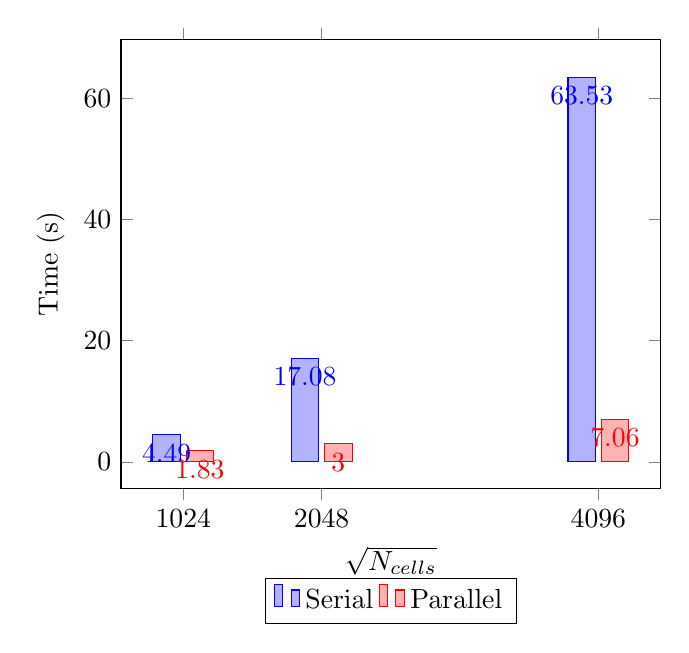
\begin{tikzpicture}
\begin{axis}[
    xlabel={$\sqrt{N_{cells}}$},
    ylabel={Time (s)},
    ybar,
    enlarge x limits=0.15,
    nodes near coords,
    nodes near coords align={vertical},
    nodes near coords style={anchor=north},
    bar width=10pt,
    xtick=data,
    xticklabels={1024, 2048, 4096},
    legend style={at={(0.5,-0.20)},anchor=north,legend columns=-1},
    ]
    \addplot coordinates {(1024,4.49401) (2048,17.0811) (4096,63.5345)};
    \addplot coordinates {(1024,1.83) (2048,3.00374) (4096,7.05673)};
    \legend{Serial, Parallel}
\end{axis}
\end{tikzpicture}
    \end{center}
    \caption{Χρόνοι εκτέλεσης της υλοποίηση με και χωρίς OpenACC.}
    \label{fig:acc_times}
\end{figure}


\subsection{Έλεγχος Αποτελεσμάτων}

Για τον έλεγχο των αποτελεσμάτων έγινε συγκρίνοντας 
την τελική κατάσταση του πίνακα των μυρμηγκιών και της φερομόνης 
μεταξύ του σειριακού κώδικα και του παραλληλοποιημένου.

% show terminal output 
\begin{lstlisting}[language=Bash]
$ diff simulation_serial.log simulation_acc.log && echo "Same!"
Same!
\end{lstlisting}

\lstinputlisting[caption=Έξοδος της προσομοίωσης για χειροκίνητο έλεγχο των αποτελεσμάτων για 2 βήματα.]{assets/simulation_serial.log}

Βλέπουμε πως η προσομοίωση έχει υλοποιηθεί σωστά αφού το μυρμήγκι κινείται στο γειτονικό κελί με τη μεγαλύτερη ποσότητα φερομόνης 
και η ποσότητα φερομόνης αλλάζει κατάλληλα.

\bibliography{bibliography}

\end{document}
